\documentclass[UTF8, 12pt]{ctexart}

\usepackage{amsmath}

\usepackage{geometry}
\geometry{a4paper, scale = 0.9} % a4纸, 版心占页面长度的比例为0.9

\usepackage{enumitem} % itemize, 列表

\usepackage{graphicx}

\begin{document}

	反向比例运算电路 :

	电路图 :

	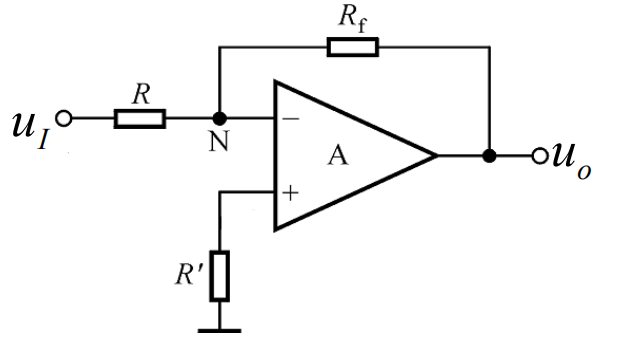
\includegraphics[scale = 0.4]{07/反向比例运算电路电路图.png}

	$ u_{o} = -\frac{R_{f}}{R}u_{i} $

	同向比例运算电路 :

	电路图 :

	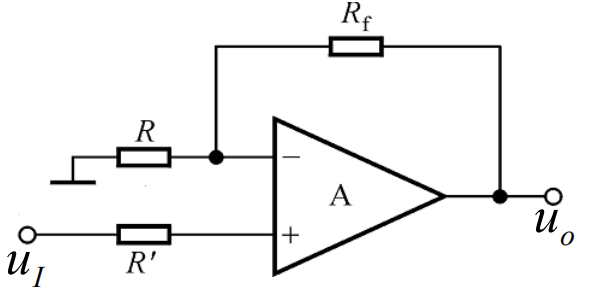
\includegraphics[scale = 0.4]{07/同向比例运算电路电路图.png}

	$ u_{o} = (1+\frac{R_{f}}{R})u_{i} $

	求和运算电路 :

	电路图 :

	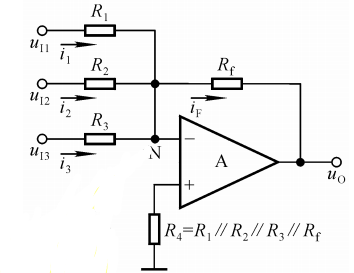
\includegraphics[scale = 0.4]{07/求和运算电路电路图.png}

	$ u_{o} = -R_{f}(\frac{u_{I1}}{R_{1}}+\frac{u_{I2}}{R_{2}}+\frac{u_{I3}}{R_{3}}) $

	加减运算电路 :

	电路图 :

	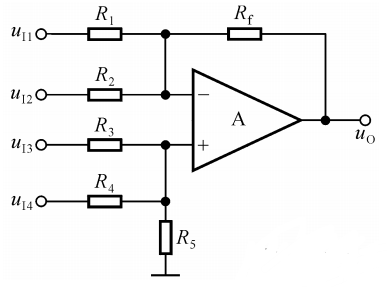
\includegraphics[scale = 0.4]{07/加减运算电路电路图.png}

	$ R_{1} \parallel R_{2} \parallel R_{f} = R_{3} \parallel R_{4} \parallel R_{5} $, $ u_{o} = R_{f}(\frac{u_{I3}}{R_{3}}+\frac{u_{I4}}{R_{4}}-\frac{u_{I1}}{R_{1}}-\frac{u_{I2}}{R_{2}}) $

	积分运算电路 :

	电路图 :

	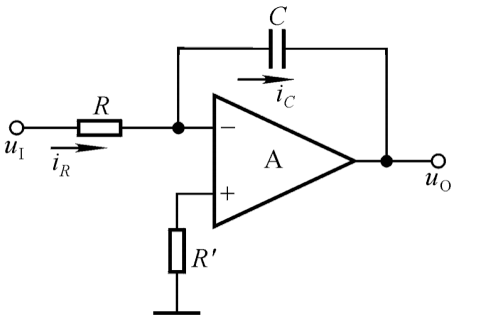
\includegraphics[scale = 0.4]{07/积分运算电路电路图.png}

	$ u_{o} = -\frac{1}{RC} \int u_{i}\mathrm{d}t $

	微分运算电路 ;

	电路图 :

	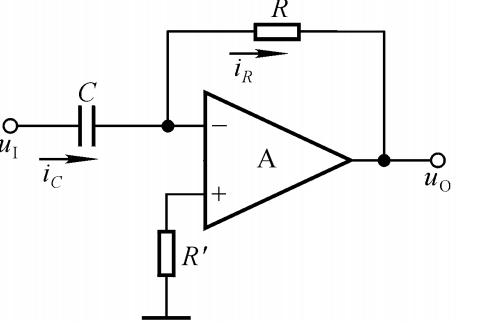
\includegraphics[scale = 0.4]{07/微分运算电路电路图.png}

	$ u_{o} = -RC\frac{\mathrm{d}u_{i}}{\mathrm{d}t} $

	~

	\noindent

	单限比较器 :

	电路图 :

	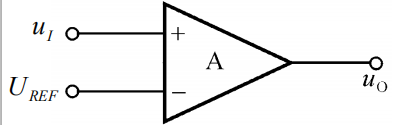
\includegraphics[scale = 0.4]{07/单限比较器电路图.png}

	特性曲线 :

	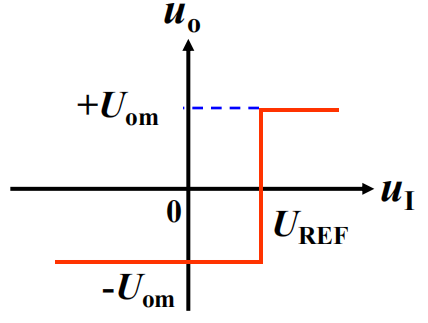
\includegraphics[scale = 0.4]{07/单限比较器特性曲线.png}

	限幅电路(输入) :

	电路图 :

	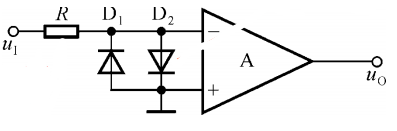
\includegraphics[scale = 0.4]{07/限幅电路(输入).png}

	限幅电路(输出) :

	电路图($ D_{z1}, D_{z2} $ 可以合并称一个管子) :

	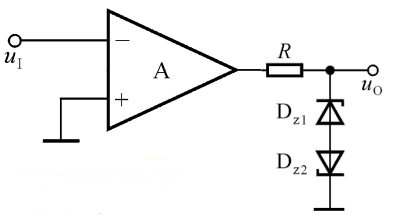
\includegraphics[scale = 0.4]{07/限幅电路(输出).png}

	滞回比较器 :

	电路图 :

	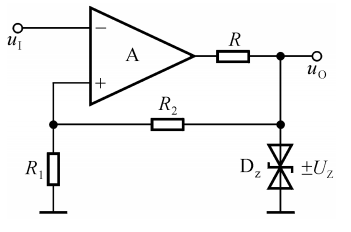
\includegraphics[scale = 0.4]{07/滞回比较器电路图.png}

	特性曲线 :

	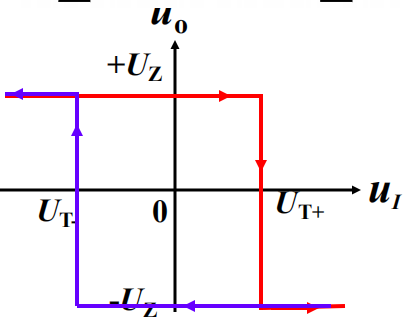
\includegraphics[scale = 0.4]{07/滞回比较器特性曲线.png}

	分析 :
	\begin{itemize}[leftmargin = 4em]
		\item $ U_{T+} = \frac{R_{1}}{R_{1}+R_{2}}U_{Z}, U_{T-} = -\frac{R_{1}}{R_{1}+R_{2}}U_{Z} $
		\item $ u_{i} $ 增大到 $ U_{T+} $ 时, 输出跳变为 $ U_{z} $, $ u_{i} $ 减小到 $ U_{T-} $ 时, 输出跳变为 $ -U_{z} $
		\item 改变 $ U_{T+}, U_{T-} $ : $ R_{1} $ 接地端改接参考电压, $ U_{T+} = \frac{R_{2}}{R_{1}+R_{2}}U_{REF} + \frac{R_{1}}{R_{1}+R_{2}}U_{Z}, U_{T-} = \frac{R_{2}}{R_{1}+R_{2}}U_{REF}-\frac{R_{1}}{R_{1}+R_{2}}U_{Z} $
	\end{itemize}

\end{document}